\chapter{Frontend}

The frontend is the core part for interaction between our PSUI and the user, which gives it little room for mistake, as we are dependent on the users interest.
When the user begins interacting with our front-end, everything sets up for a session dependent on the users choice.
Either guest or private mode can be selected.
If the guest mode is chosen then a non saving session will get started, where the user gets the experience answering questions,
genereted by our localy saved llm.
Reaching a state, where the user is pleased and does not want to continue answering questions anymore, the session can either be closed or a personal grading can be requested.
If previously private mode was chosen instead of guest mode, then the users efforts will be saved on server side, so return users can continue where they left of answering.
After terminating the session the next user can get in line and start answering questions.

\section{General Setup}


\section{URL Routing}
For URL navigation, we decided to use file based routing, which is a common practice in modern web applications.
In our specific case, we used the TanStack Router library.
This approach allows us to modularize our application into clear and structured URLs.
We can clearly define which component is in use, when a certain URL is accessed, which makes the code better maintainable and more understandable.


\section{Main Screen}
\begin{figure}[H]
    \centering
    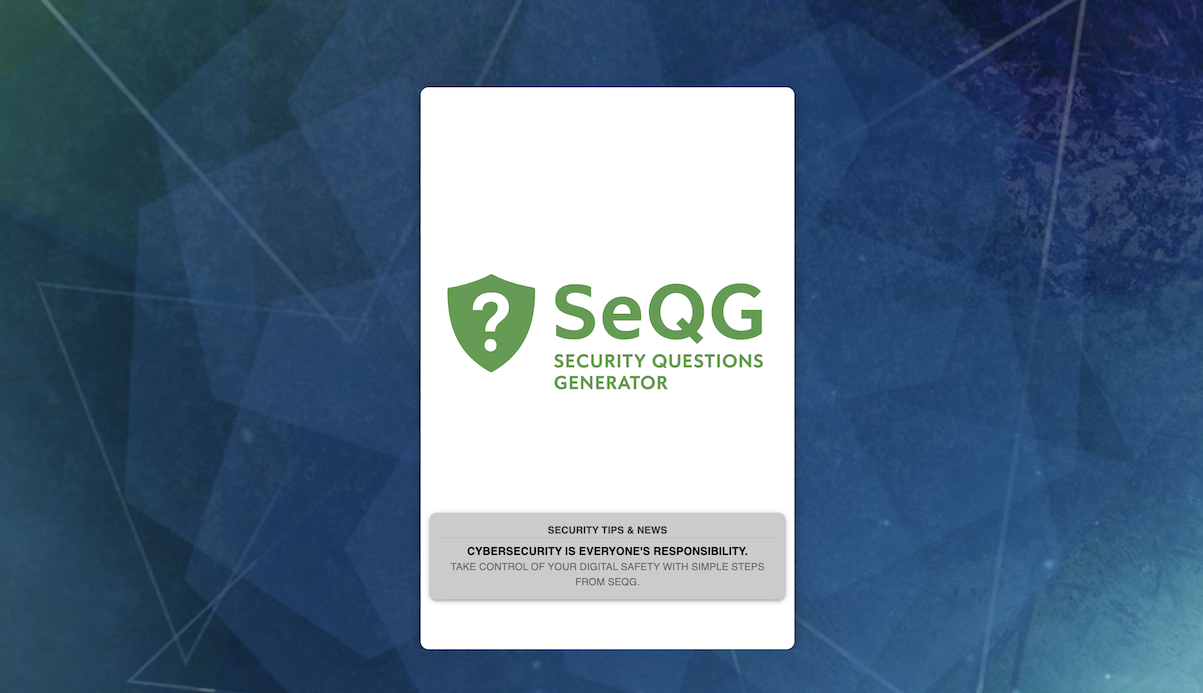
\includegraphics[width=0.8\textwidth]{images/MainScreen1.png}
    \caption{Main Screen}
\end{figure}

When the system is offline, the display shows a static screen where \textbf{security tips and news} are 
dynamically fetched by the LLM. These messages, shown in Figure 2.1, are designed to catch users’ attention 
and encourage them to engage with \textbf{SeQG} and learn more about \textbf{cybersecurity}.

\begin{figure}[H]
    \centering
    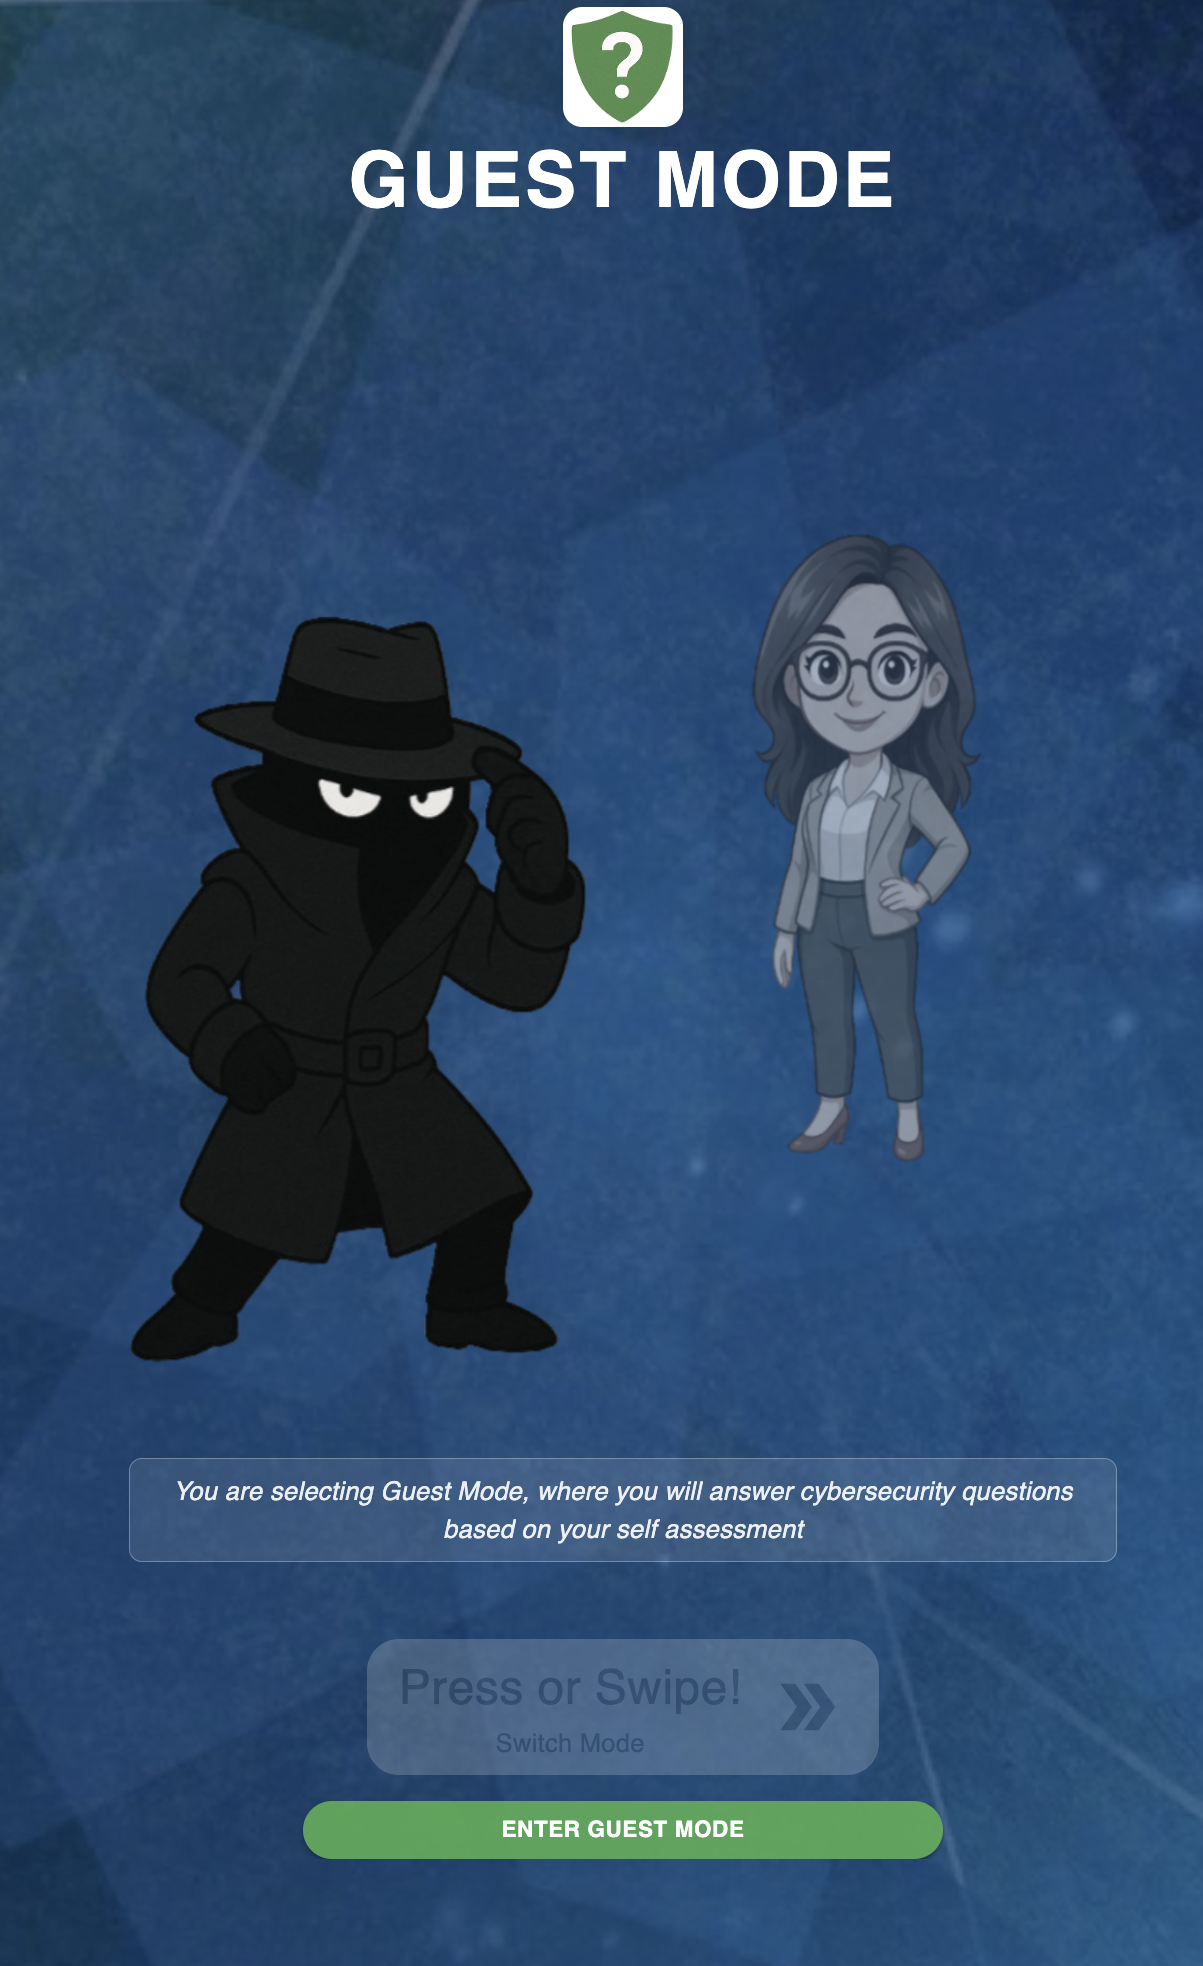
\includegraphics[width=0.4\textwidth]{images/MainScreenCharacter1.png}
    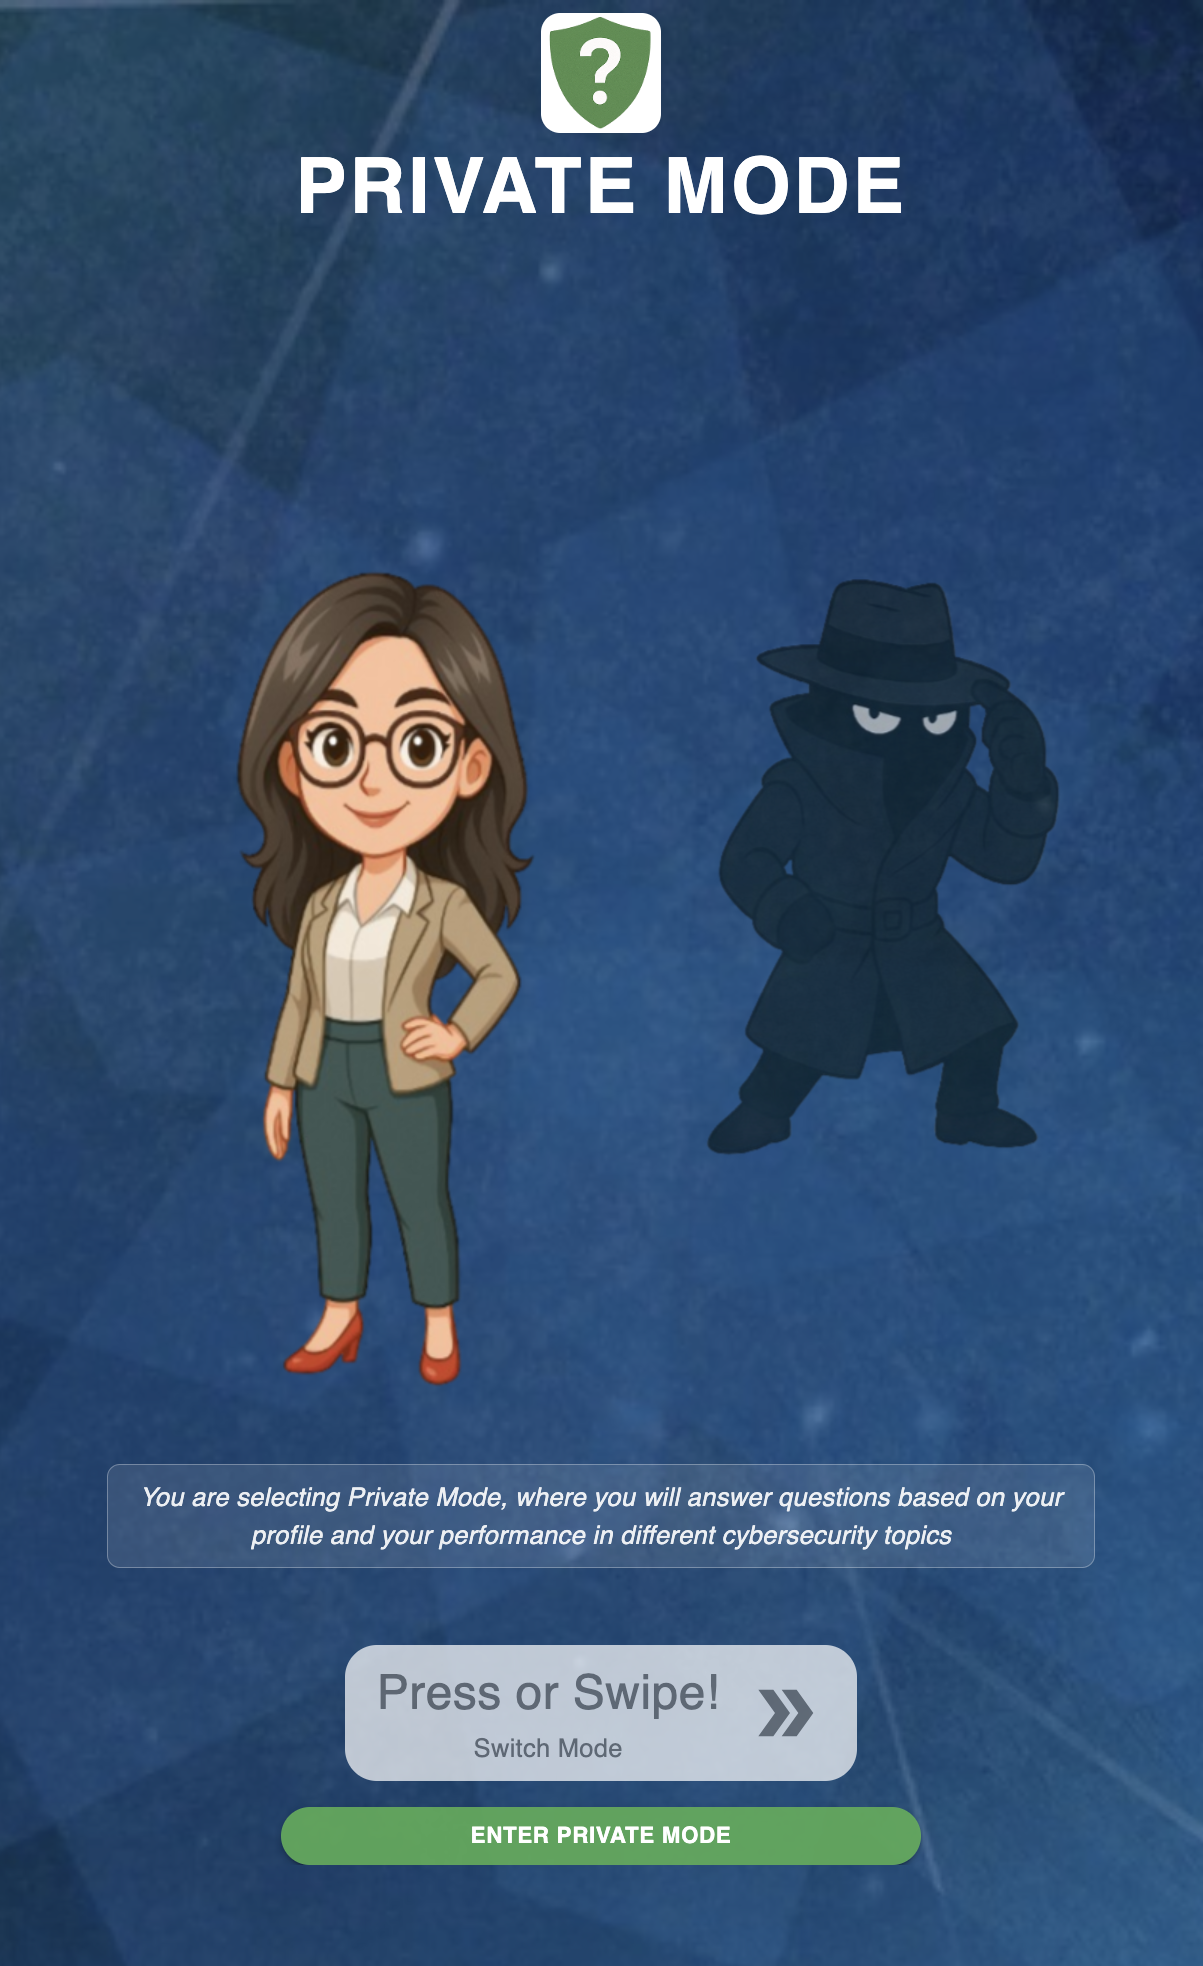
\includegraphics[width=0.4\textwidth]{images/MainScreenCharacter2.png}
    \caption{Characters for Mode selection}
\end{figure}
When a user approaches the display and taps the screen, \textbf{two mode characters} appear, each accompanied 
by a short explanation of their functionality, as to be seen in Figure 2.3.
\section{Welcome Screens}

\begin{figure}[H]
    \centering
     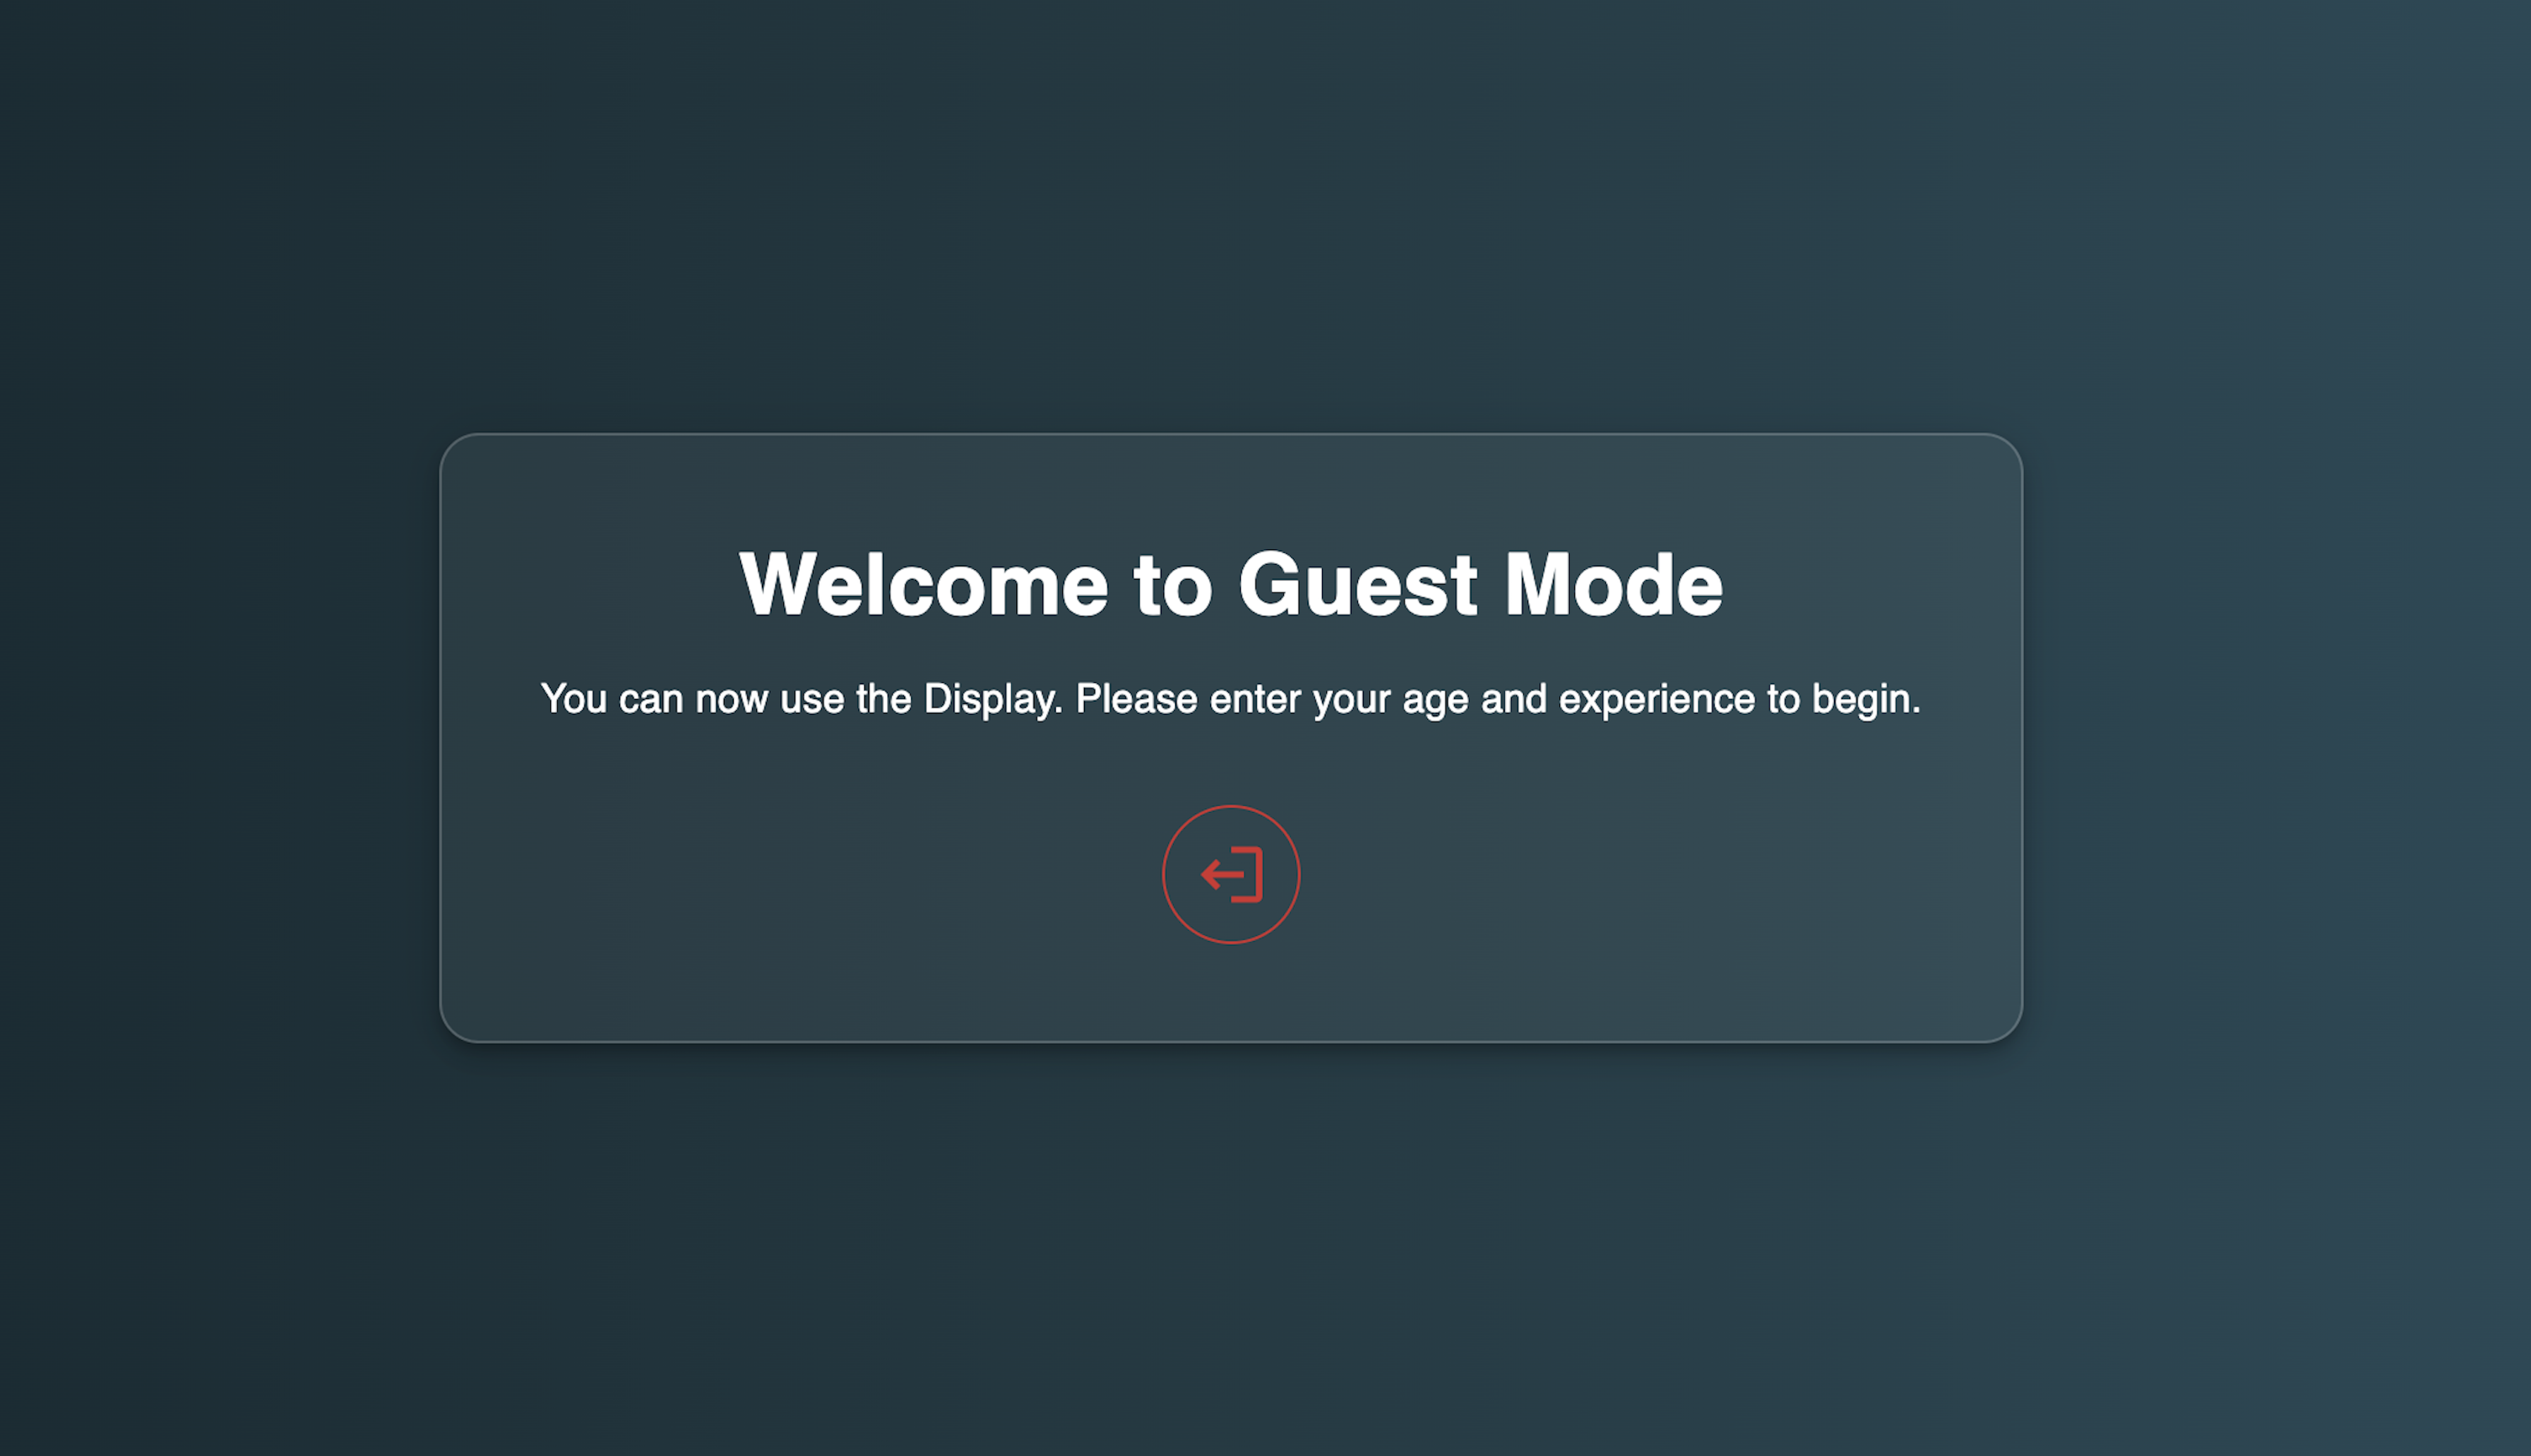
\includegraphics[width=0.6\textwidth]{images/WelcomeScreen.png}
     \caption{Main When connected}
\end{figure}
When the user scans the QR code with their device, a screen will appear allowing them to leave the 
session remotely without needing to interact directly with the public display. While connected, 
a \textbf{session token} linked to the user's device is stored on the server, preventing other 
users from interfering with the session.

\begin{figure}[H]
    \centering
    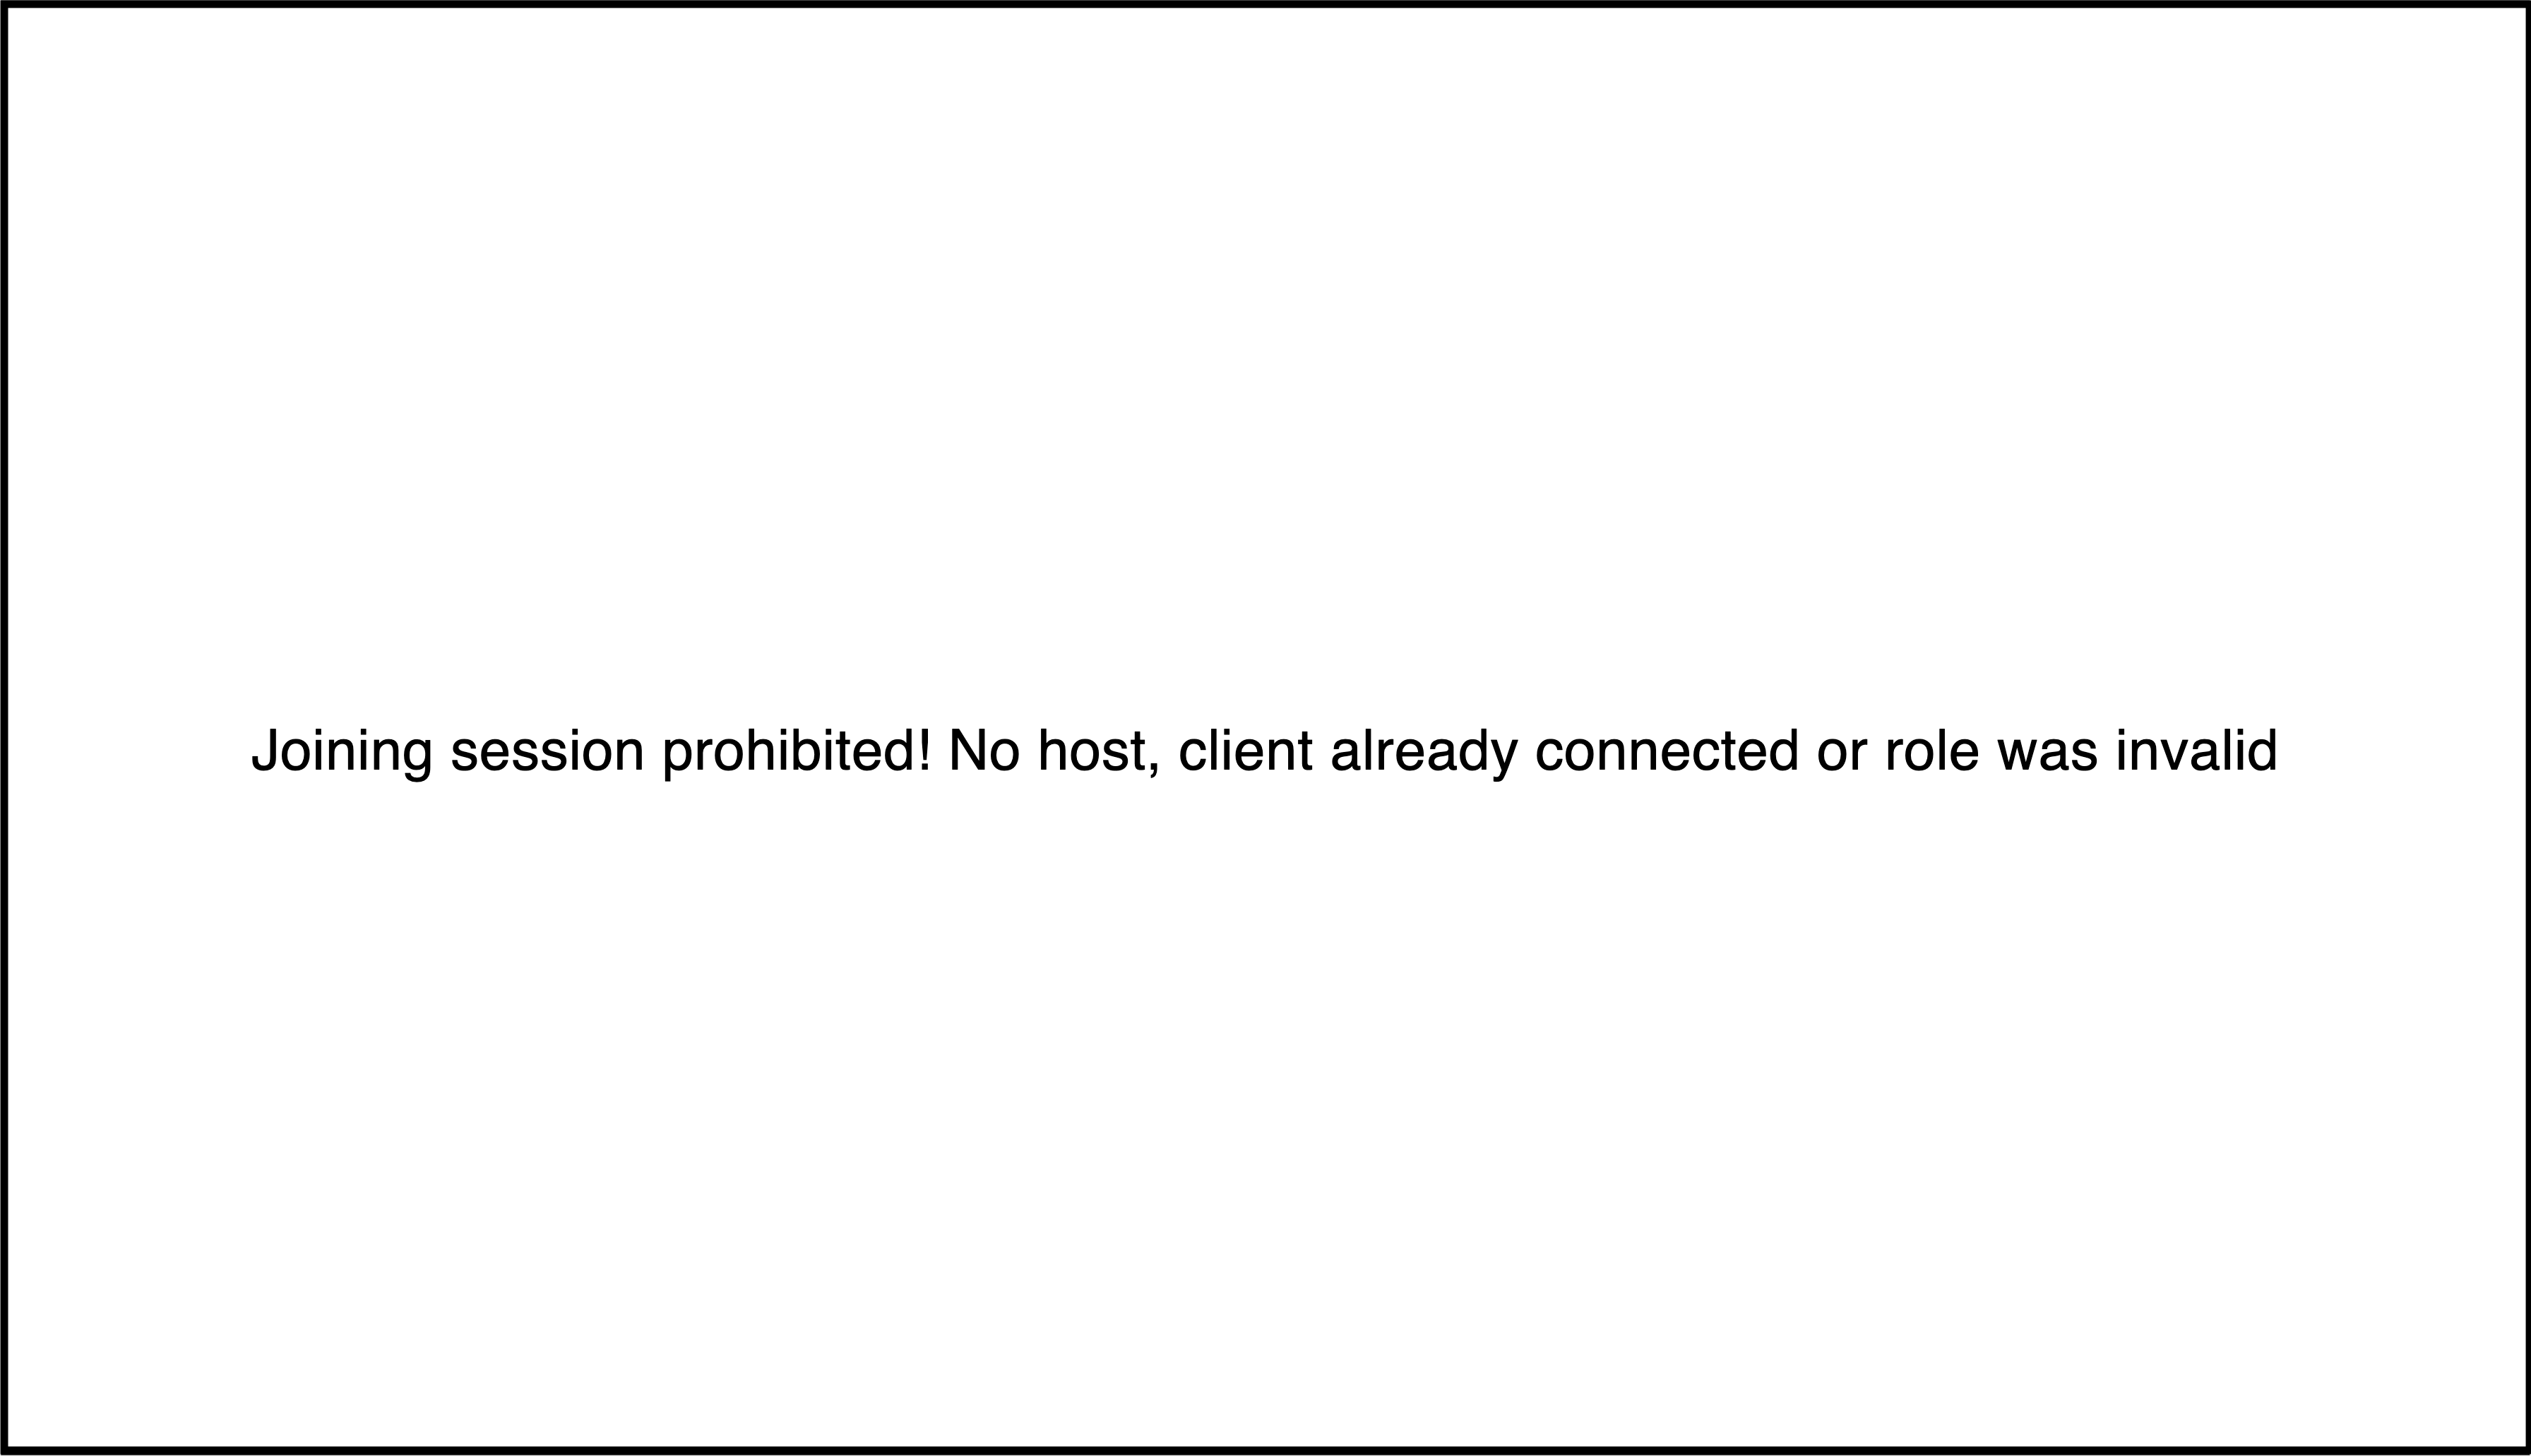
\includegraphics[width=0.6\textwidth]{images/WelcomeScreenInvalid.png}
    \caption{When trying to connect}
\end{figure}
If a user is already connected to the server, any subsequent user who scans the QR code will see 
a different screen on their device, informing them that the \textbf{session is currently occupied}.
\section{Modes}

\subsection{QR Code - Integration}
QR codes play a central role in how devices connect within \textbf{SeQG}. 
They are used as a simple and intuitive way to link a user's device to an active session. 
When a session is started, the application generates a QR code containing a unique link. 
This link includes a hidden session identifier that tells the system, which session the user can connect to.
Once scanned, the device opens the link, which automatically redirects the user to the corresponding session within the app. 
The beauty of this process is that it requires almost no effort from the user, as no code or password is required. 
Everything happens in just a few seconds by scanning the QR code.

\subsection{Communication with Backend}
The \textbf{SeQG} frontend communicates with the backend through WebSockets to enable real-time, bidirectional data exchange. 
Here we differentiate between client and host frontend.
The host frontend must stay in constant connection with the backend, while a session is active, whereas the client frontend needs to connect only once. 
Before the client can connect, the host frontend must first request a JWT token and then connect to the backend with this token.
As the user joins a session, the client's frontend uses the previously fetched JWT token from the host's frontend and connects to the backend, via the URL saved in the QR Code. 
While connecting, the client's frontend emits an ''register'' event containing:
\begin{itemize}
    \item the token from the URL
    \item a role
    \item the user's unique ID from localStorage (if private-mode)
\end{itemize}
If the session is valid and the user is allowed to join, they're granted access and the interaction begins. 
If not, they receive a ''already\_connected'' message, which can then be handled as an invalid user.
This approach makes it easy to manage users in real time.
\subsection{Guest Mode}
Guest Mode is designed for quick, one-time participation without any setup or login. 
It allows users to access a session instantly without any user data being stored. 
When someone joins a session in Guest Mode, the application automatically generates a temporary user identity and stores it locally in the browser. 
This identity helps the system recognize the user during the session. 
Guest users have full access to participate in the session’s activities, but their presence is temporary and not tied to any personal information. 
Once the session ends or the browser is closed, the user effectively disappears from the system’s memory.
This mode is ideal for situations where users are not expected to return.

\subsection{Private Mode}
Private Mode offers a more structured and secure way to connect to a session. 
It is used when a user scans a QR code that links to a specific, private session. 
This link contains a hidden token that identifies the session and grants access to it. 
When the user opens the link, the application uses this token to establish a secure connection with the backend system. 
At the same time, the user's device is assigned a unique identifier, which is stored locally and remains available for future sessions on the same device. 
This allows the system to recognize returning users, maintain a consistent identity across multiple sessions, and apply session-specific rules or roles. 
The connection is verified before granting access — so users without the correct token or link will be blocked.
\subsection{Question Types}
SeQG has \textbf{six question types implemented}, enhancing the user's gamified experience with a dynamic, entertaining
app. Each of these question types has been implemented with visual animations depending on the correctness of
the answer and each one of them has an explanation generated by the LLM in case the user answered incorrectly.
The six question types are:
\begin{itemize}[nosep]
    \item \textbf{Single choice} 
    \item \textbf{Multiple choice} 
    \item \textbf{Think event} 
    \item \textbf{Drag \& drop}
    \item \textbf{Sorting}
    \item \textbf{Line-connect}
\end{itemize}

\pagebreak
\subsubsection{Single choice}
In this question type, the user is offered \textbf{two possible solutions} and has to select the correct answer. Once they
touch on the desired answer, the correct answer will be highighted in green. If they have failed, an instant LLM explanation
will be fetched on the same screen for the user to learn:
\begin{figure}[htbp]
    \centering
    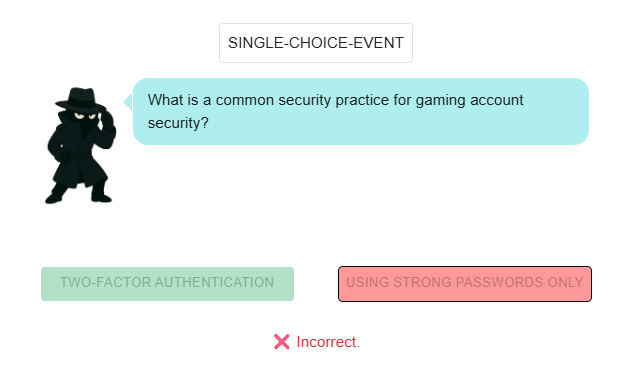
\includegraphics[width=0.5\textwidth]{images/Single_Choice.png}
\end{figure}

\subsubsection{Multiple choice}
Here the user is given \textbf{between two and four possible solutions} and has to select \textbf{all} correct answers. Once every
correct asnwer is selected, the must press the submit button:
\begin{figure}[htbp]
    \centering
    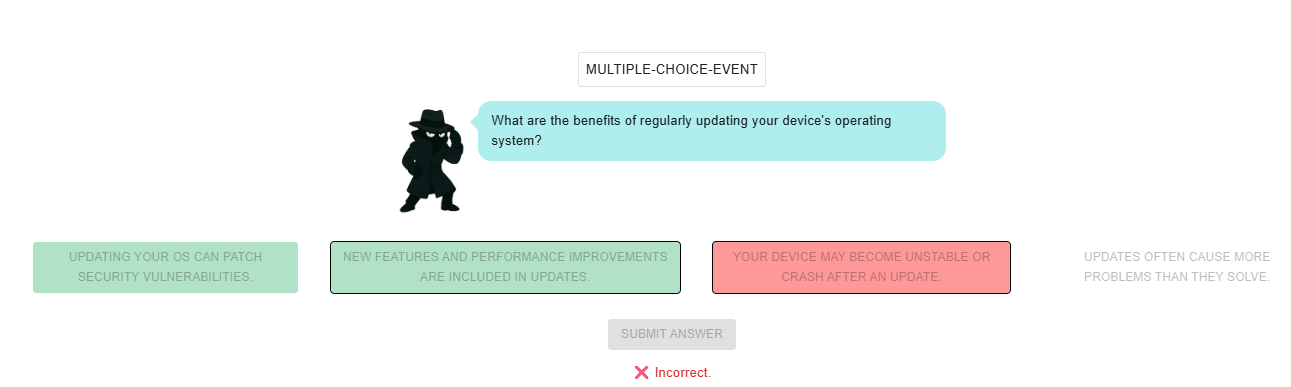
\includegraphics[width=1\textwidth]{images/Multiple_Choice.png}
\end{figure}

\subsubsection{Think Event}
In the think event, the user must think about the possible answer to the question formulated for \textbf{fifteen seconds}. Once the
time is up, they must (honestly) select whether they knew the correct answer or not:
\begin{figure}[htbp]
    \centering
    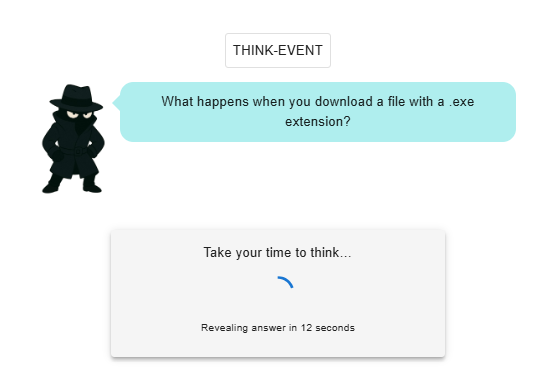
\includegraphics[width=0.45\textwidth]{images/Think_Event.png}
    \hfill
    \raisebox{-5mm}{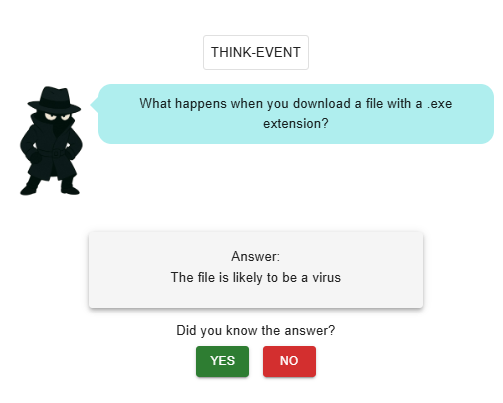
\includegraphics[width=0.45\textwidth]{images/Think_Event_2.png}}
\end{figure}
\pagebreak

\subsubsection{Drag \& Drop}
The user must drag the boxes into the \textbf{correct category}. There is also the possibility to revert the answer:
\begin{figure}[htbp]
    \centering
    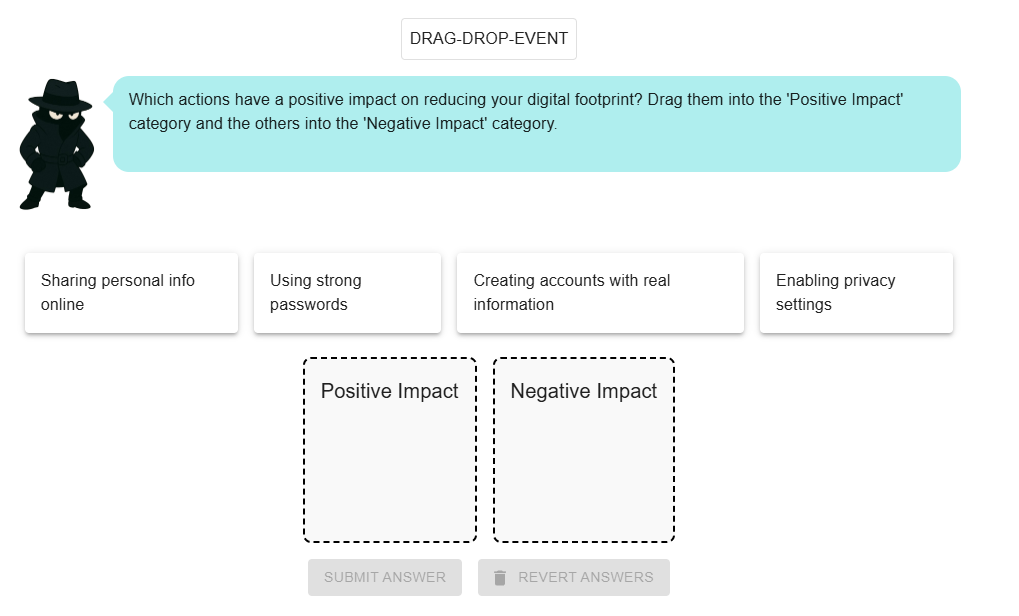
\includegraphics[width=0.8\textwidth]{images/Drag_and_Drop.png}
\end{figure}

\subsubsection{Sorting}
All the answers must be \textbf{correctly sorted}. As before, the user can return to the original order whenever they want:
\begin{figure}[htbp]
    \centering
    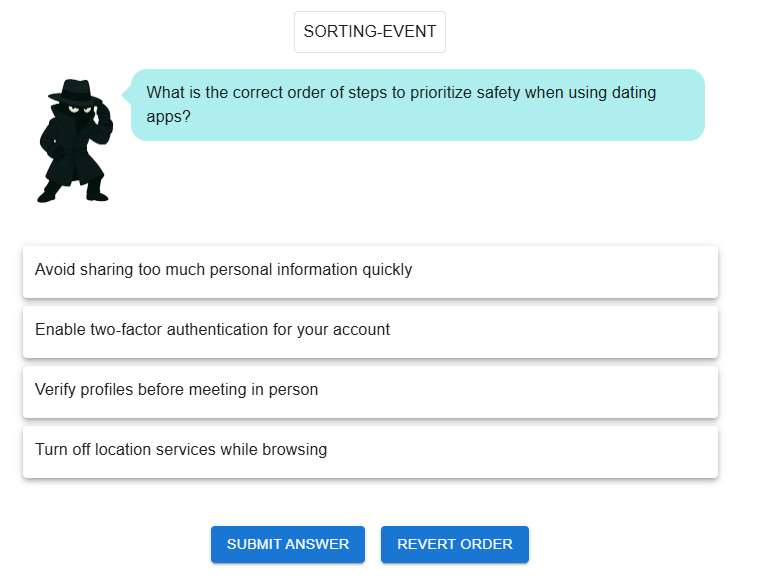
\includegraphics[width=0.6\textwidth]{images/Sorting.png}
\end{figure}
\pagebreak

\subsubsection{Line-connect}
In tis question type \textbf{an even number} of boxes is displayed, having to match each item on one side to their correspondant
on the other side. There is also the answer reversal button to start again:
\begin{figure}[htbp]
    \centering
    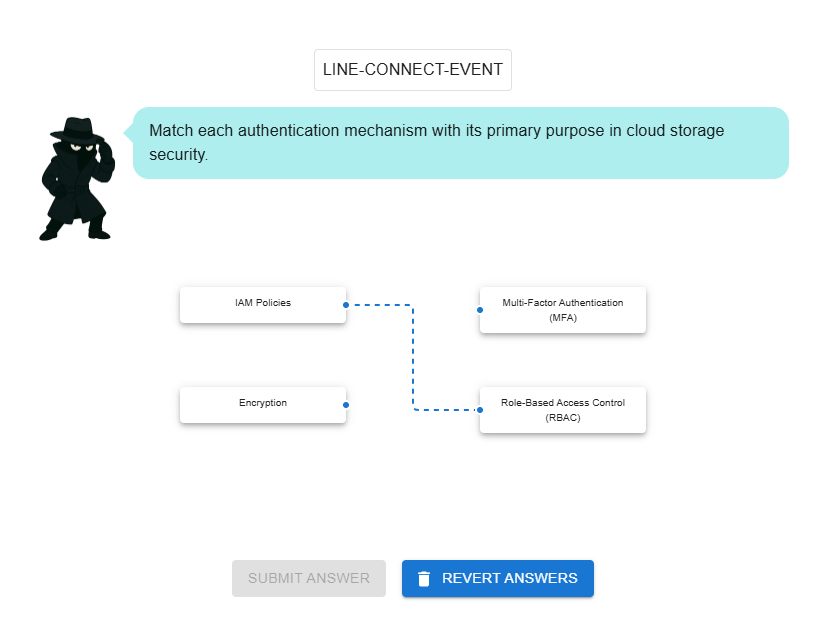
\includegraphics[width=0.8\textwidth]{images/Line_Connect.png}
\end{figure}

\subsection{Gradings}

When the user finishes their session (in both guest and private modes), a dashboard appears summarizing their \textbf{performance}. 
To enhance user feedback and engagement in SeQG, the dashboard includes radar charts assessing the user's performance 
across each specific \textbf{cybersecurity topic}, generated with Chart.js. The diagram is split into two if there are more 
than eight topics, to avoid exceeding the visual limit. The dashboard also includes \textbf{personalized feedback}, as 
shown in Figure 2.5, which highlights the user's strengths and weaker areas during their session, encouraging 
them to use SeQG again to improve their \textbf{cybersecurity awareness}. User Progress is persistently stored in a 
structured JSON format if the user started a private session, including metadata such as their userID, age, 
experience and per-topic experience.

\begin{figure}[H]
    \centering
    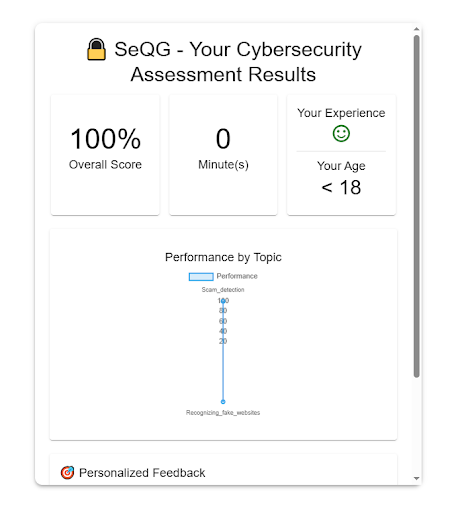
\includegraphics[width=0.4\textwidth]{images/Grading2.png}
    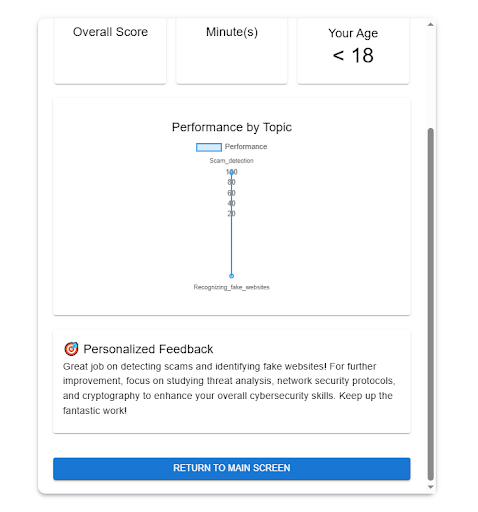
\includegraphics[width=0.4\textwidth]{images/Grading3.png}
    \caption{Dashboard}
\end{figure}

The interface also includes an inactivity timer that triggers a message in the center of the screen after 60 seconds 
of \textbf{no interaction}. The user then has 10 seconds to confirm their presence; otherwise, the session is closed and the 
system returns to the main screen.

\begin{figure}[H]
    \centering
    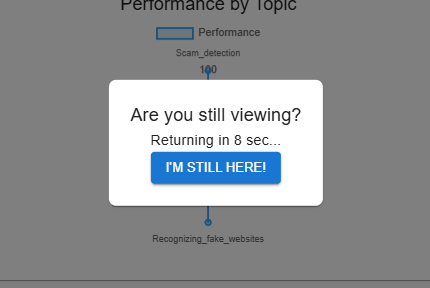
\includegraphics[width=0.35\textwidth]{images/Grading1.png}
    \caption{Inactivity timer pop-up message}
\end{figure}